\documentclass[11pt, a4paper] {article}
\usepackage[czech]{babel}
\usepackage[utf8]{inputenc}
\usepackage{xurl}
\usepackage{csquotes}
\usepackage[czech]{babel}
\usepackage[utf8]{inputenc}
\usepackage[left=2cm, top=3cm, text={17cm, 24cm}]{geometry}
\usepackage{times}
\usepackage{xcolor}
\usepackage{float}
\usepackage{graphicx}
\graphicspath{ {img/} }
\usepackage{verbatim}
\usepackage[unicode]{hyperref}

\begin{document}
    
    \begin{titlepage}
        \begin{center}
        \Huge
        \textsc{Vysoké učení technické v Brně\\
        \huge
        {Fakulta informačních technologií}\\} 
        \vspace{\stretch{0.382}}
        \LARGE
        IMP projekt \\
        \Huge{Řízení dopravní křižovatky} \\
        \LARGE
        \vspace{\stretch{0.1}}
        Jiří Kotek: xkotek09@stud.fit.vutbr.cz \\
        \vspace{\stretch{0.518}}
        \end{center} 
        {\Large \today \hfill
        }
    \end{titlepage}

    %\tableofcontents

    %\newpage

    %%%%%%%%%%%%%%%%%%%%%%%%%%%%%%%%%%%%%%%%%%%%%%%%%%%%%%%%%%%%%%%%%%%%%%%%%%%%%%%%%%%%%%%%%%%%%%%%
    %% ÚVOD A MOOTIVACE
    \section{Úvod}
        V tomto projektu je cílem  navrhnout a implementovat program pro řízení dopravní křižovatky 
        ve tvaru T se třemi přechody pro chodce. 

        Cílová platforma je vývojová deska FRDM-KL27Z obsahující mikrokontroler MKL27Z64VLH4.
    %%%%%%%%%%%%%%%%%%%%%%%%%%%%%%%%%%%%%%%%%%%%%%%%%%%%%%%%%%%%%%%%%%%%%%%%%%%%%%%%%%%%%%%%%%%%%%%%
    %% KONCEPCE PŘÍSTUPU, MODELU
    \section{Návrh}
        V rámci řízení modelu bude potřebovat rozlišovat hlavní tři stavy, ve kterém se systém nachází.

        \begin{figure}[H]
            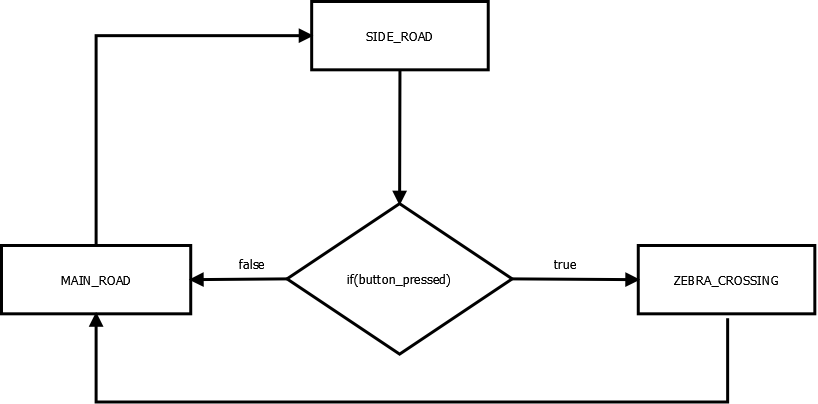
\includegraphics[width=0.8\textwidth]{diagramNavrh.png}
            \centering
            \caption{Návrh modelu řízení křižovatky.}
            \label{Navrh}
        \end{figure}

        \begin{itemize}
            \item stav: \verb|MAIN_ROAD|: Stav, ve kterém bude signál volno na hlavní silnici.
            \item stav: \verb|SIDE_ROAD|: Stav, ve kterém bude signál volno na vedlejší silnici.
            \item stav: \verb|ZEBRA_CROSSING|: Stav, ve kterém bude umožněno chodcům přejít křižovatku.
        \end{itemize}

        Okamžik stiknutí tlačítka budeme zaznamenávat pomocí přerušení. Pro časování jednotlivých přechodů mezi stavy
        využijeme vestavěný modul RTC (angl. Real Time Clock). 

        Přídavná světla u semaforů řídících provoz vozidel nebudou využita. Jejich využití při rozlišení
        dvou stavů by bylo matoucí.


    %%%%%%%%%%%%%%%%%%%%%%%%%%%%%%%%%%%%%%%%%%%%%%%%%%%%%%%%%%%%%%%%%%%%%%%%%%%%%%%%%%%%%%%%%%%%%%%%
    %% IMPLEMENTACE MODELU
    \section{Implementace}
        Aplikace při spuštění a vkročení do hlavní funkce \verb|main| nejprve provede inicialiuaci hardwaru pomocí funkce \verb|HW_init()|.
        Tato funkce byla již předefinována prostředím MCUXpresso. Následně je volána\\ funkce \verb|Port_Init()|, která
        povolí rozvod hodinového signálu na potřebné porty a nastaví, které piny jsou vstupní, které výstupní.

        Dále je zavolána funkce \verb|Button_interrupt_init()|, která povolí vyvolání přerušení 
        při sestupné hraně signálu stisku tlačítka. Před povolením přerušení v modulu NVIC (Nested Vector Interrupt Controller),
        jsou případná předchozí přerušení z portu B smazána pomocí \verb|NVIC_ClearPendingIRQ()|.

        Program využívá vestavěného modulu RTC. Tento modul je inicializován ve funkci \verb|RTC_init()|. V rámci této funkce je 
        povolen rozvod hodin, zvolení 32kHz oscilátoru, nastavení prescaleru a povolení zachycení přerušení v modulu NVIC.

        Po nastavení veškerého hardwaru funkce \verb|main()| vchází do nekonečné smyčky, ve které zůstává po zbytek běhu.
        Průběh nastavení, je znázorněn na obrázku~\ref{vyvojDia}
        \begin{figure}[H]
            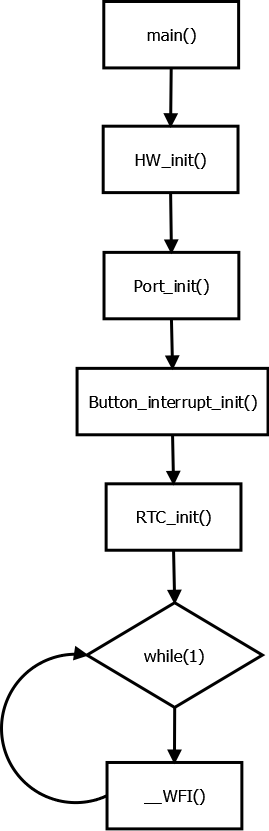
\includegraphics[width=0.3\textwidth]{vyvojDia.png}
            \centering
            \caption{Vývojový diagram znázorňující průběh nastavovení mikrokontroleru ve funkci main. Instrukce WFI()
            zajišťuje vyčkání na přerušení při využití minima zdrojů.}
            \label{vyvojDia}
        \end{figure}

        Řízení křižovatky (tj. rozsvicování a zhásínání světelných signálů) je realizováno pomocí konečného automatu~\ref{Automat}.

        \begin{figure}[H]
            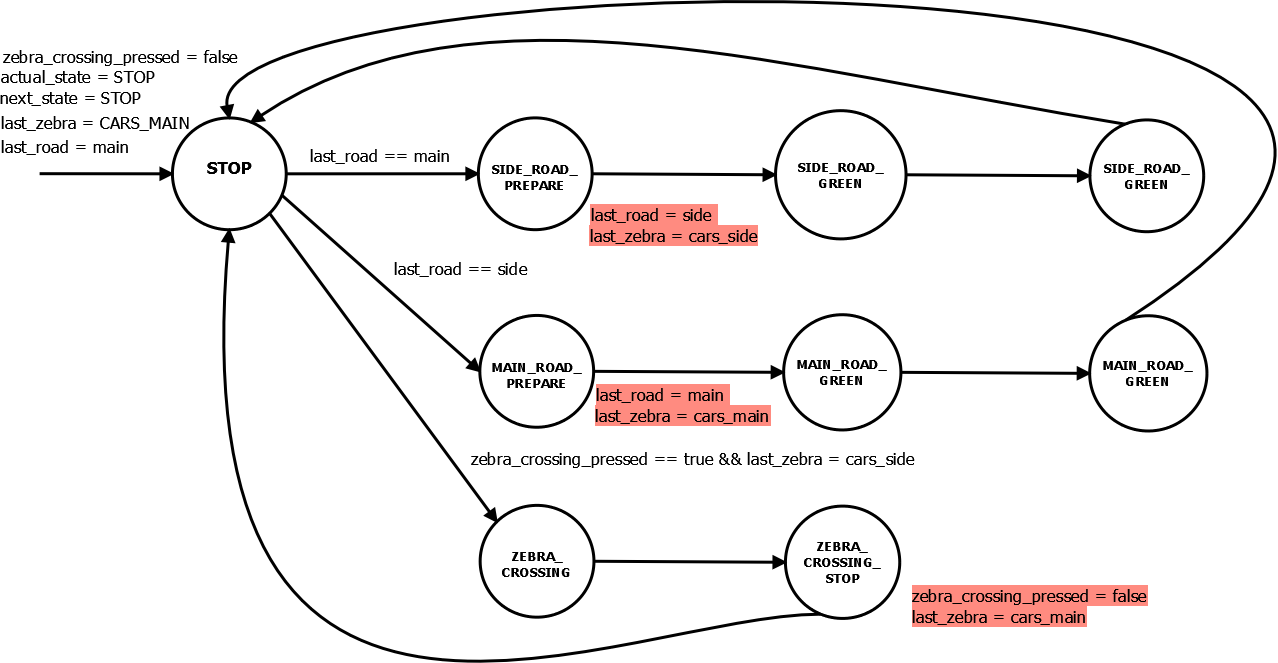
\includegraphics[width=1.0\textwidth]{IMPautomat.png}
            \centering
            \caption{Moorův konečný automat realizující řízení křižovatky. Výstup stavů je pro zpřehlednění umítěn vždy 
            vpravo od stavu, ke kterému se vztahuje a označen červeným pozadím. Při vstupu do automatu jsou vyznačeny
            výchozí hodnoty proměnných.}
            \label{Automat}
        \end{figure}

        Přechod mezi stavy je realizován pomocí časovaného přerušení. Nastavení konkrétních intervalů setrvání
        je možné nastavit ve funkci \verb|state_timer()|.

        Pro přesun mezi stavy využívám dvě hlavní pomocné proměnné \verb|actual_state| a \verb|next_state|, do níž 
        ukládám aktuální a následující stav.  

        Proměnná \verb|zebra_crossing_pressed| je nastavena na hodnotu \verb|true| v případě vyvolání přerušení stisku tlačítka.
        Proměnná \verb|last_road| si pamatuje, které z cest byla uvolněna jako poslední. Nabývá hodnot \verb|SIDE| nebo \verb|MAIN|.
        Proměnná \verb|last_zebra| slouží k ošetření případu, kdy by chodec neutále vyvolával požadavek pro přechod silnice a 
        program by tak neustále poutěl chodce donekonečna.

    %%%%%%%%%%%%%%%%%%%%%%%%%%%%%%%%%%%%%%%%%%%%%%%%%%%%%%%%%%%%%%%%%%%%%%%%%%%%%%%%%%%%%%%%%%%%%%%%
    %% ZÁVĚR
    \section{Závěr}
        V rámci projektu bylo implementováno jednoduché řízení křižovatky ve tvaru T. Program střídavě
        uvolněje provoz mezi hlavní a vedlejší cestou. V případě stisku tlačítka pro chodce 
        je po skončení cyklu provoz zastven a na všech přechodech se zobrazí zelená. 

        Projekt by mohl být v budoucnu rozšířen pro využití přídavných světel. Jejich využití
        ovšem spatřuji pouze v případě, kdy by byla zelená zobrazena vždy pouze v jednom ze tří směrů.

        Odkaz na demonstrační video se nachází v souboru README.md

    %%%%%%%%%%%%%%%%%%%%%%%%%%%%%%%%%%%%%%%%%%%%%%%%%%%%%%%%%%%%%%%%%%%%%%%%%%%%%%%%%%%%%%%%%%%%%%%%
    %% ZDROJE
    %\newpage
    %\section{Zdroje}
    %    \bibliographystyle{czechiso}
	%  \bibliography{imp-proj}


\end{document}